\documentclass[11pt,aspectratio=1610]{beamer}
\usepackage{fbb}
\usetheme{CambridgeUS}
\beamertemplatenavigationsymbolsempty
\usepackage[utf8]{inputenc}
\usepackage{amsmath,adjustbox,mathtools}
\usepackage{amsfonts}
\usepackage{hyperref}
\usepackage{graphicx}
\usepackage{xpatch}
\usepackage{makecell}
\usepackage{tabularx}
\usepackage{csquotes}
\usepackage{adjustbox}
\setbeamertemplate{caption}{\raggedright\insertcaption\par}
\usepackage{minted}
\usetheme{default}
\usecolortheme{default}


% Définition des couleurs
\definecolor{schTag}{RGB}{204, 0, 0}       % Rouge pour les balises
\definecolor{schAttr}{RGB}{0, 0, 153}      % Bleu pour les attributs
\definecolor{schValue}{RGB}{0, 102, 0}     % Vert pour les valeurs
\definecolor{schBg}{RGB}{245, 245, 245}    % Fond gris clair

% Configuration de minted
\setminted{
  bgcolor=schBg,
  frame=single,
  framesep=3mm,
  linenos=False,
  breaklines=true,
  fontsize=\small,
}


\usepackage{pgfplots}
\usepackage{tikz}
\usetikzlibrary{shapes,calc,matrix,decorations.markings,decorations.pathreplacing,positioning, intersections,backgrounds,through,hobby}
\usepackage[english]{babel}
%\AtBeginSection[]
%{\begin{frame}
% \frametitle{}  
%\setlength{\itemsep}{.5cm}
% \tableofcontents[currentsection,
%                  hideothersections,
%		  sectionstyle=hide/hide/hide,
%                  subsectionstyle=show/show/show/hide
%                   ]
% \end{frame} 
% }

%\AtBeginsection[]
%{\begin{frame}
% \frametitle{}  
% \tableofcontents[currentsection,
%	 	  currentsection,
%		  sectionstyle=show/hide,
%                  sectionstyle=show/shaded/hide
%                   ]
% \end{frame} 
% }


\AtBeginSection[]
{
  \begin{frame}
    \tableofcontents[
      currentsection,       % Met en évidence la section courante
      sectionstyle=show/shaded, % Sections : courante en évidence, autres en grisé
      subsectionstyle=hide  % Cache toutes les sous-sections
    ]
  \end{frame}
}
 
 

\AtBeginSubsection[]
{
  \begin{frame}
    \tableofcontents[
     currentsection, % Affiche uniquement la section courante
      hideothersubsections, % Cache les sous-sections des autres sections
      sectionstyle=show/hide, % Cache les autres sections
      subsectionstyle=show/shaded/hide % Sous-section courante en évidence, les autres en grisé
    ]
  \end{frame}
}


\setbeamertemplate{sections/subsections in toc}[square]
\setbeamertemplate{bibliography item}[sqare]
\setbeamertemplate{itemize item}[square]
\setbeamertemplate{enumerate item}[square]
\setbeamertemplate{itemize subitem}[square]




\setbeamertemplate{sections/sections in toc}[square]
\setbeamertemplate{itemize item}[square]
\setbeamertemplate{enumerate item}[square]
\setbeamertemplate{itemize subitem}[square]

\usepackage[style=verbose,citestyle=authoryear,isbn=true,url=false,
doi=true,backend=biber,maxbibnames=9, maxcitenames=4]{biblatex}
\addbibresource{/home/mgl/Bureau/Travail/Communications_et_articles/bibliographie_commune/biblio.bib}
\renewcommand*{\bibfont}{\tiny} 

\usepackage{tikz}
\usetikzlibrary{shapes,calc,matrix,decorations.markings,decorations.pathreplacing,positioning, intersections,backgrounds}
\tikzstyle{bag} = [align=center]

\date[24 mars 2026]{24 mars 2026}
\author[Matthias \textsc{Gille Levenson}]{\\~\\ Matthias \textsc{Gille Levenson}\\   {\scriptsize Université Versailles Saint Quentin (UVSQ) \& École Normale Supérieure de Lyon, France}\\ {\tiny matthias [dot] gille [-] levenson [at] ens-lyon [dot] fr}\vspace{-1cm}}
\title[La TEI]{Session II: la TEI\\ {\small Atelier Humanités Numériques \\ Lyon}}
%\titlegraphic{\hspace{0.5cm}\includegraphics[scale=0.21]{/home/mgl/Bureau/Travail/admin/logos/ensl.png}\hspace{0.5cm}\includegraphics[scale=0.23]{/home/mgl/Bureau/Travail/admin/logos/ciham.pdf}\hspace{0.5cm}}
\usepackage[justification=centering]{caption}
\begin{document}
\maketitle

\section{Organisation de la TEI}

\subsection{Éléments et attributs}

\begin{frame}{Éléments proposés par la TEI}
\begin{itemize}
\item La TEI propose d'utiliser un certain nombre d'éléments définis en amont. 
\item Faire de la TEI, c'est utiliser ce jeu d'éléments pour décrire un objet textuel.
\item Exemples: l'élément \texttt{div} est utilisé pour indiquer une section, soit une division structurelle du texte. L'élément \texttt{p} est utilisé pour identifier des paragraphes dans des textes en prose. 
\end{itemize}
\end{frame}

\begin{frame}[containsverbatim]{Représenter l'incipit de la \textit{Recherche}}
La \textit{Recherche} est structurée en tomes, eux-même divisés en parties et en chapitres.
\begin{minted}[breaklines,numbersep=10mm]{xml}
<div>
    <div>
        <p>Longtemps, je me suis couché de bonne heure 
        [...]
        </p>
    </div>
</div>
\end{minted}
\end{frame}

\begin{frame}{Attributs proposés par la TEI}
\begin{itemize}
\item Chaque élément peut être précisé par un attribut.
\item Ces attributs (sauf ceux qui commencent par \texttt{`xml:`}) sont également spécifiques à la TEI
\item Exemple: \texttt{n} est un attribut permettant de compter un élément (un vers, par exemple, ou un chapitre)

\end{itemize}
\end{frame}

\begin{frame}[containsverbatim]{L'utilisation d'attributs propres à la TEI}
\begin{minted}[breaklines,numbersep=10mm]{xml}
<div n="1">
    <div n="1">
        <p>Longtemps, je me suis couché de bonne heure 
        [...]
        </p>
    </div>
</div>
\end{minted}
\end{frame}

\begin{frame}{Attributs proposés par la TEI}
\begin{itemize}
\item Nous avons souvent besoin de préciser et de classer les différents éléments
\item La TEI propose un attribut \texttt{type} pour ce faire
\end{itemize}
\end{frame}

\begin{frame}[containsverbatim]{L'utilisation d'attributs propres à la TEI}
\begin{minted}[breaklines,numbersep=10mm]{xml}
<div n="1" type="partie">
    <div n="1" type="chapitre">
        <p>Longtemps, je me suis couché de bonne heure 
        [...]
        </p>
    </div>
</div>
\end{minted}
\end{frame}

\subsection{Des objets définis et illustrés}
\begin{frame}
\begin{itemize}
\item La TEI ne se limite pas à proposer une liste d'éléments et d'attributs
\item Il est nécessaire de les définir afin de favoriser leur utilisation
\item Chaque élément et chaque attribut est ainsi défini dans les Guidelines
\item Taper \enquote{\texttt{TEI element}} sur votre moteur de recherche favori vous mène directement à la définition de l'élément \texttt{element} cherché.
\end{itemize}
\end{frame}


\begin{frame}{Exemple: \texttt{p}}
\begin{itemize}
\item L'élément p est défini ici: \href{https://www.tei-c.org/release/doc/tei-p5-doc/fr/html/ref-p.html}{https://www.tei-c.org/release/doc/tei-p5-doc/fr/html/ref-p.html}
\end{itemize}
\end{frame}

\begin{frame}
\begin{figure}
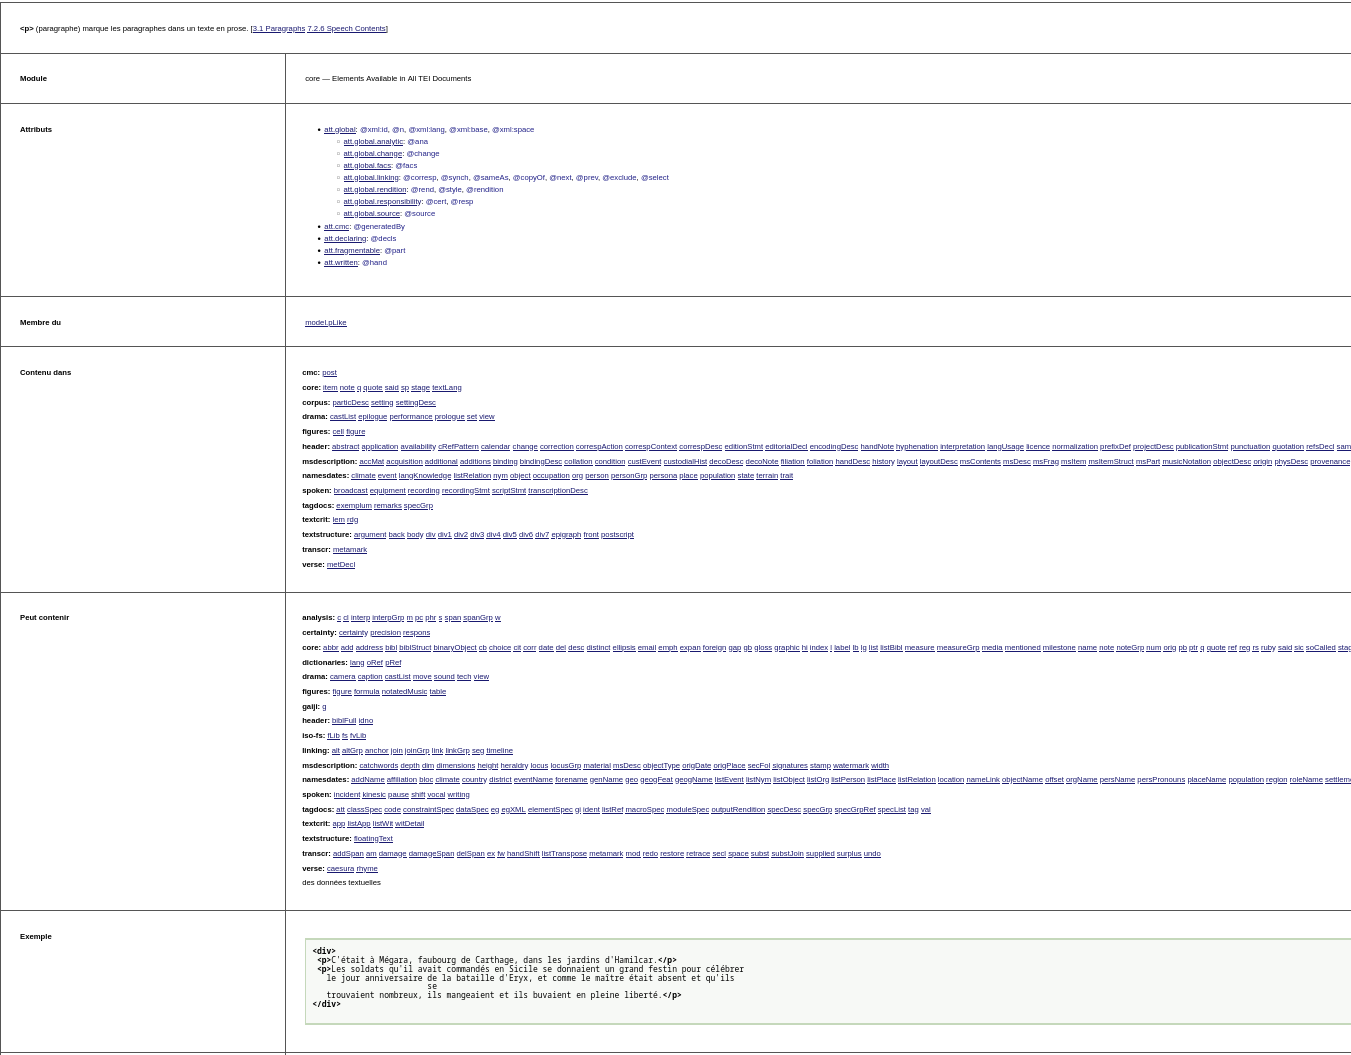
\includegraphics[height=.8\textheight]{../../img/definition_p.png}
\end{figure}
\end{frame}

\begin{frame}{Ce que contient une page décrivant un élément}
La page contient: 
\begin{enumerate}
\item Une définition avec un renvoi vers le \textbf{module} correspondant (voir plus bas)
\item La liste des attributs autorisés
\item La définition selon le modèle de la TEI 
\item Les éléments qui peuvent contenir l'élément courant
\item Les éléments contenus dans l'élément courant
\item Un exemple et un lien vers une liste d'exemples d'utilisation de l'élément
\end{enumerate}
\end{frame}


\begin{frame}{Exemple: \texttt{p}}
La page contient: 
\begin{enumerate}
\item Il est nécessaire d'aller lire la définition d'un élément avant de l'utiliser
\item Il est quasi-certain qu'il existe déjà un élément pour votre besoin
\item Ne réinventez pas la roue !
\end{enumerate}
\end{frame}

\subsection{Les modules thématiques}

\subsection{Qu'est-ce qu'un module?}
\begin{frame}
\begin{itemize}
\item Un module est un chapitre des \textit{Guidelines} qui vient décrire un thème spécifique
\item Chaque module est décrit en langage naturel et vient présenter des cas typiques d'encodage.
\item Avant de commencer un projet, il faut avoir lu les modules correspondants afin de faire les meilleurs choix possibles.
\end{itemize}
\end{frame}

\subsection{Modules fondamentaux}

\begin{frame}{Les métadonnées et le \texttt{teiHeader}}
\begin{itemize}
\item Un document XML-TEI est composé au minimum de deux parties: les métadonnées et l'objet décrit.
\item Les métadonnées, qui décrivent le document en lui-même (auteur.e, source, régime de publication, année, etc), sont renseignées dans la première partie, le \texttt{teiHeader}
\end{itemize}
\end{frame}

\begin{frame}{Structure textuelle}
\begin{itemize}
\item Les divisions sont marquées par \texttt{div} ou \texttt{div1, div2, div3}. Le choix entre les deux est obligatoire !
\item Les paragraphes de la prose, par \texttt{p}
\item Les sections moins claires sémantiquement peuvent être indiquées par \texttt{ab} (anonymous block)
\end{itemize}
\end{frame}

\begin{frame}{Représentation des sources primaires}
\begin{itemize}
\item
\end{itemize}
\end{frame}

\begin{frame}{Entités nommées}
\begin{itemize}
\item
\end{itemize}
\end{frame}

\begin{frame}{Description de manuscrits}
\begin{itemize}
\item
\end{itemize}
\end{frame}

\begin{frame}{Apparats critiques}
\begin{itemize}
\item
\end{itemize}
\end{frame}





\section{Application: encoder des vers et du théâtre}
\subsection{Le vers}
\begin{frame}[containsverbatim]{Les formes versifiées}
\begin{itemize}
\item Le module de la TEI est: \href{Verse}{https://tei-c.org/release/doc/tei-p5-doc/en/html/VE.html}
\item les éléments fondamentaux sont le vers (\texttt{l} pour \textit{line}), le groupe de vers (\texttt{lg} pour \textit{LineGroup})
\item Vous pouvez représenter une unité textuelle (poème) par comme un \texttt{lg} ou plus classiquement une division. 
\item L'hémistiche ou le pied peuvent être indiqués à l'aide de l'élément \texttt{seg} qui devra être précisé par un attribut \texttt{type}
\item Vous pouvez décrire la rime avec l'attribut \texttt{rhyme}, et la structure métrique avec \texttt{met}:

\begin{minted}[breaklines,numbersep=2mm]{xml}
<l>
 <seg type="foot" met="+--">Arma vi</seg>
 <seg met="+--">rumque ca</seg>
 <seg met="++">no Tro</seg>
 <seg met="++">iae qui </seg>
 <seg met="+--">primus ab</seg>
 <seg met="++"> oris</seg>
</l>
\end{minted}
\end{itemize}
\end{frame}


\begin{frame}{Encoder un sonnet}
\begin{itemize}
\item Encodez le sonnet 
\item Utilisez la spécification \texttt{TEI All} (nous y reviendrons dans la session 3)
\item Commencez par renseigner les métadonnées minimales
\item Encodez la structure du poème en considérant qu'il fait partie d'un recueil plus vaste
\item Renseignez le type de strophe et de vers à l'aide d'attributs
\end{itemize}
\end{frame}


\subsection{Le théâtre}
\begin{frame}{Le théâtre}
\begin{itemize}
\item Le module de la TEI est: \href{Performance texts}{https://tei-c.org/release/doc/tei-p5-doc/en/html/DR.html}
\item les éléments fondamentaux sont la division structurelle (similaire à \textit{supra}), les interventions des personnages (\texttt{sp})
\item Les didascalies sont encodées avec \texttt{stage}. Les mouvements des personnages, avec \texttt{move}
\item La liste des personnages se décrit à l'aide de \texttt{castList} et de \texttt{castItem}, le lieu de l'action avec \texttt{set}.
\end{itemize}
\end{frame}

\begin{frame}{Encoder un fragment d'\oe uvre dramatique}
\begin{itemize}
\item Encodez la scène finale de l'\textit{Avare} (\texttt{session\_2\_la\_tei/exercices/avare\_a5\_sc6.txt})
\item Utilisez la spécification \texttt{TEI Drama}
\item Commencez par renseigner les métadonnées minimales
\item Encodez la structure du texte en considérant qu'il fait partie d'une \oe uvre complète
\end{itemize}
\end{frame}


\begin{frame}{References}
\printbibliography
\end{frame}

\end{document}
